\section{\secondtitle}

\def\secondtitleF{Predicting learned-cuts}
\def\secondtitleS{Applying learned-cuts to the MFMP}


\begin{frame}
\frametitle{\textbf{Contents}}
  \setbeamercovered{transparent}
  \begin{block}{\textbf{\secondtitleF}}
  \end{block}  

  \only<1>{
    \begin{block}{\textbf{\secondtitleS}}
    \end{block}  
  }
  \only<2->{
    \transparent{0.3}
    \begin{block}{\textbf{\secondtitleS}}
    \end{block}  
    \transparent{1}
  }

\end{frame}

\begin{frame}
\frametitle{\textbf{Predicting learned-cuts}}
 
  % \onslide<1->{
  %   \textbf{Input data $x$}
  % }
  \onslide<2->{
  % \begin{block}{Given an optimization problem}
  %   \begin{equation*}
  %     y^{*}(x) :\equiv arg \,\,\min_{y \in \mathcal{Y}(x)} C(x,y)
  %   \end{equation*}
  % \end{block}
  \begin{columns}[c]
    \column{0.5\linewidth}
    \textbf{Optimization problem}
    \column{0.5\linewidth}
    \begin{equation*}
      y^{*}(x) :\equiv arg \,\,\min_{y \in \mathcal{Y}(x)} C(x,y)
    \end{equation*}
  \end{columns}
  }
  \onslide<3->{
  \begin{columns}[c]
    \column{0.5\linewidth}
    \textbf{Input features}
    \column{0.5\linewidth}
    \begin{equation*}
      H(x) = h_m(y) \,\, \forall m \in \mathcal{M}
    \end{equation*}
  \end{columns}
  }
  \onslide<4->{
  \begin{columns}[c]
    \column{0.5\linewidth}
    \textbf{Solution features}
    \column{0.5\linewidth}
    \begin{equation*}
      G(y) = g_n(y) \,\, \forall n \in \mathcal{N}
    \end{equation*}
  \end{columns}
  }
  \onslide<6->{
  \begin{columns}[c]
    \column{0.5\linewidth}
    \textbf{Training for optimal}
    \column{0.5\linewidth}
    \begin{equation*}
      G(y^*(x)) \approx \hat{G}(x) = f(H(x))
    \end{equation*}
  \end{columns}
  }
  % TODO: example.
  \only<2>{
   \begin{adjustbox}{max totalsize={.5\textwidth}{.5\textheight},center}
      \DrawSolution{none}{none}{0}
   \end{adjustbox}
  }
  \only<3-4>{
   \begin{adjustbox}{max totalsize={.5\textwidth}{.5\textheight},center}
      \DrawSolution{gy}{none}{0}
   \end{adjustbox}
  }
  \only<5->{
   \begin{adjustbox}{max totalsize={.5\textwidth}{.5\textheight},center}
      \DrawSolution{gyoptim}{none}{0}
   \end{adjustbox}
  }

\end{frame}

\begin{frame}
\frametitle{\textbf{Applying learned-cuts}}
  \onslide<2->{
  \begin{columns}[c]
    \column{0.6\linewidth}
    \textbf{We predict the optimal features}
    \column{0.4\linewidth}
    \begin{equation*}
      \hat{G}(x) = \hat{g}_n(x) \,\, \forall n \in \mathcal{N}
    \end{equation*}
  \end{columns}
  }
  \onslide<3->{
  \begin{columns}[c]
    \column{0.6\linewidth}
    \textbf{We predict the optimal ``zone''}
    \column{0.4\linewidth}
    \begin{align*}
      & \mathcal{Y}^\prime(x) = \{y \in \mathcal{Y} \mid  \hat{G}(x) = G(y) \}
    \end{align*}
  \end{columns}
  }
  \onslide<4->{
  \begin{columns}[c]
    \column{0.6\linewidth}
    \textbf{We solve the predicted model}
    \column{0.4\linewidth}
    \begin{equation*}
      \hat{y}^{*}(x) :\equiv arg \,\,\min_{y \in \mathcal{Y}^\prime(x)} C(x,y)          
    \end{equation*}
  \end{columns}
  }
  \onslide<5->{
    \begin{columns}[c]
      \column{0.6\linewidth}
      \textbf{With some (hopefully small) loss :}
      \column{0.4\linewidth}
      \begin{equation*}
        C(x,\hat{y}^{*}(x)) \approx  C(x,y^{*}(x))
      \end{equation*}
    \end{columns}
    }

  \only<1>{
   \begin{adjustbox}{max totalsize={.5\textwidth}{.5\textheight},center}
      \DrawSolution{none}{none}{0}
   \end{adjustbox}
  }
  \only<2>{
   \begin{adjustbox}{max totalsize={.5\textwidth}{.5\textheight},center}
      \DrawSolution{ghat}{none}{0}
   \end{adjustbox}
  }
  \only<3>{
   \begin{adjustbox}{max totalsize={.5\textwidth}{.5\textheight},center}
      \DrawSolution{ghat}{north west lines}{0}
   \end{adjustbox}
   }
  \only<4>{
   \begin{adjustbox}{max totalsize={.5\textwidth}{.5\textheight},center}
      \DrawSolution{ghat}{north west lines}{1}
   \end{adjustbox}
   }
  \onslide<5->{
   \begin{adjustbox}{max totalsize={.5\textwidth}{.5\textheight},center}
      \DrawSolution{ghat}{north west lines}{2}
   \end{adjustbox}
   }
\end{frame}

% \begin{frame}
% \frametitle{\textbf{Optimality of learned-cuts}}

%   \begin{columns}[c]
%     \column{0.6\linewidth}
%     \textbf{With some (hopefully small) loss :}
%     \column{0.4\linewidth}
%     \begin{equation*}
%       C(x,\hat{y}^{*}(x)) \approx  C(x,y^{*}(x))
%     \end{equation*}
%   \end{columns}
%   \only<1>{
%    \begin{adjustbox}{max totalsize={.5\textwidth}{.5\textheight},center}
%       \DrawSolution{ghat}{north west lines}{1}
%    \end{adjustbox}
%    }
%   \only<2->{
%    \begin{adjustbox}{max totalsize={.5\textwidth}{.5\textheight},center}
%       \DrawSolution{ghat}{north west lines}{2}
%    \end{adjustbox}
%    }
%    % TODO: legend
% \end{frame}

\begin{frame}
\frametitle{\textbf{Contents}}
  \setbeamercovered{transparent}
  \transparent{0.3}
  \begin{block}{\textbf{\secondtitleF}}
  \end{block}  
  \transparent{1}

  \begin{block}{\textbf{\secondtitleS}}
  \end{block}  
\end{frame}

\begin{frame}
\frametitle{\textbf{Motivation}}
  
  \pause
  \begin{enumerate}[<+->]

  \item
    \textbf{Performance}: a smaller model is easier to solve.
  \item
    \textbf{User feedback}: direct feedback about the solution without
    needing to solve any model.
  \item
    \textbf{Apply secondary objectives}: Filter solutions taking into account other more intractable criteria.
  \end{enumerate}
\end{frame}

\begin{frame}
\frametitle{\textbf{New formulation}}

% TODO: legend, aircraft i, period t, M= check
  \only<2>{
  \begin{tabular}{p{5mm}p{90mm}}
    $a_{ijtt'}$ & : aircraft $i$ is in mission $j$ between $t$ and $t'$.  \\
  \end{tabular}
  }
  \onslide<3->{
  \begin{tabular}{p{5mm}p{90mm}}
    $a_{ijtt'}$ & : aircraft $i$ is in mission $j$ between $t$ and $t'$.  \\
    $m_{ip}$ &: aircraft $i$ uses check pattern $p$. \\
  \end{tabular}
  }

  \onslide<5->{
    \begin{align}
      & \sum_{(j, t, t') \in \mathcal{J}\mathcal{T}\mathcal{T}_{ic}} a_{ijtt'} H^\prime_{jtt'} + U^{\prime}_{tc} \leq H^{M} + bigM (1 - m_{ip}) & \notag \\
      & \hspace{200px}  i \in \mathcal{I}, p \in \mathcal{P}, c \in \mathcal{C}_p \notag
    \end{align}
  }

  \only<1>{
    \DrawGantt{0}{0}{0}
  }
  \only<2>{
    % missions
    \DrawGantt{0}{1}{0}
  }
  \only<3>{
    % maintenances and missions
    \DrawGantt{2}{1}{0}
  }
  \only<4->{
    % maints, missions and cycles
    \DrawGantt{2}{1}{cycle}
  }
\end{frame}

\begin{frame}
\frametitle{\textbf{Solution feature: distance between maintenances}}

  For each aircraft $i$: $D_i(y) \in [E^{min},E^{max}] \,\, \forall y \in \mathcal{Y}(x)$. \\
  \onslide<3->{
    Solution feature: $g_1(y) = \mu_{t'-t} = \frac {\sum_{i \in \mathcal{I}} D_i(y)}{I}$. \\
  }
  \only<2-3>{
    \DrawGantt{2}{0}{distance}
  }
  \only<4->{
    Distribution of $\mu^*_{t'-t}$: \\
  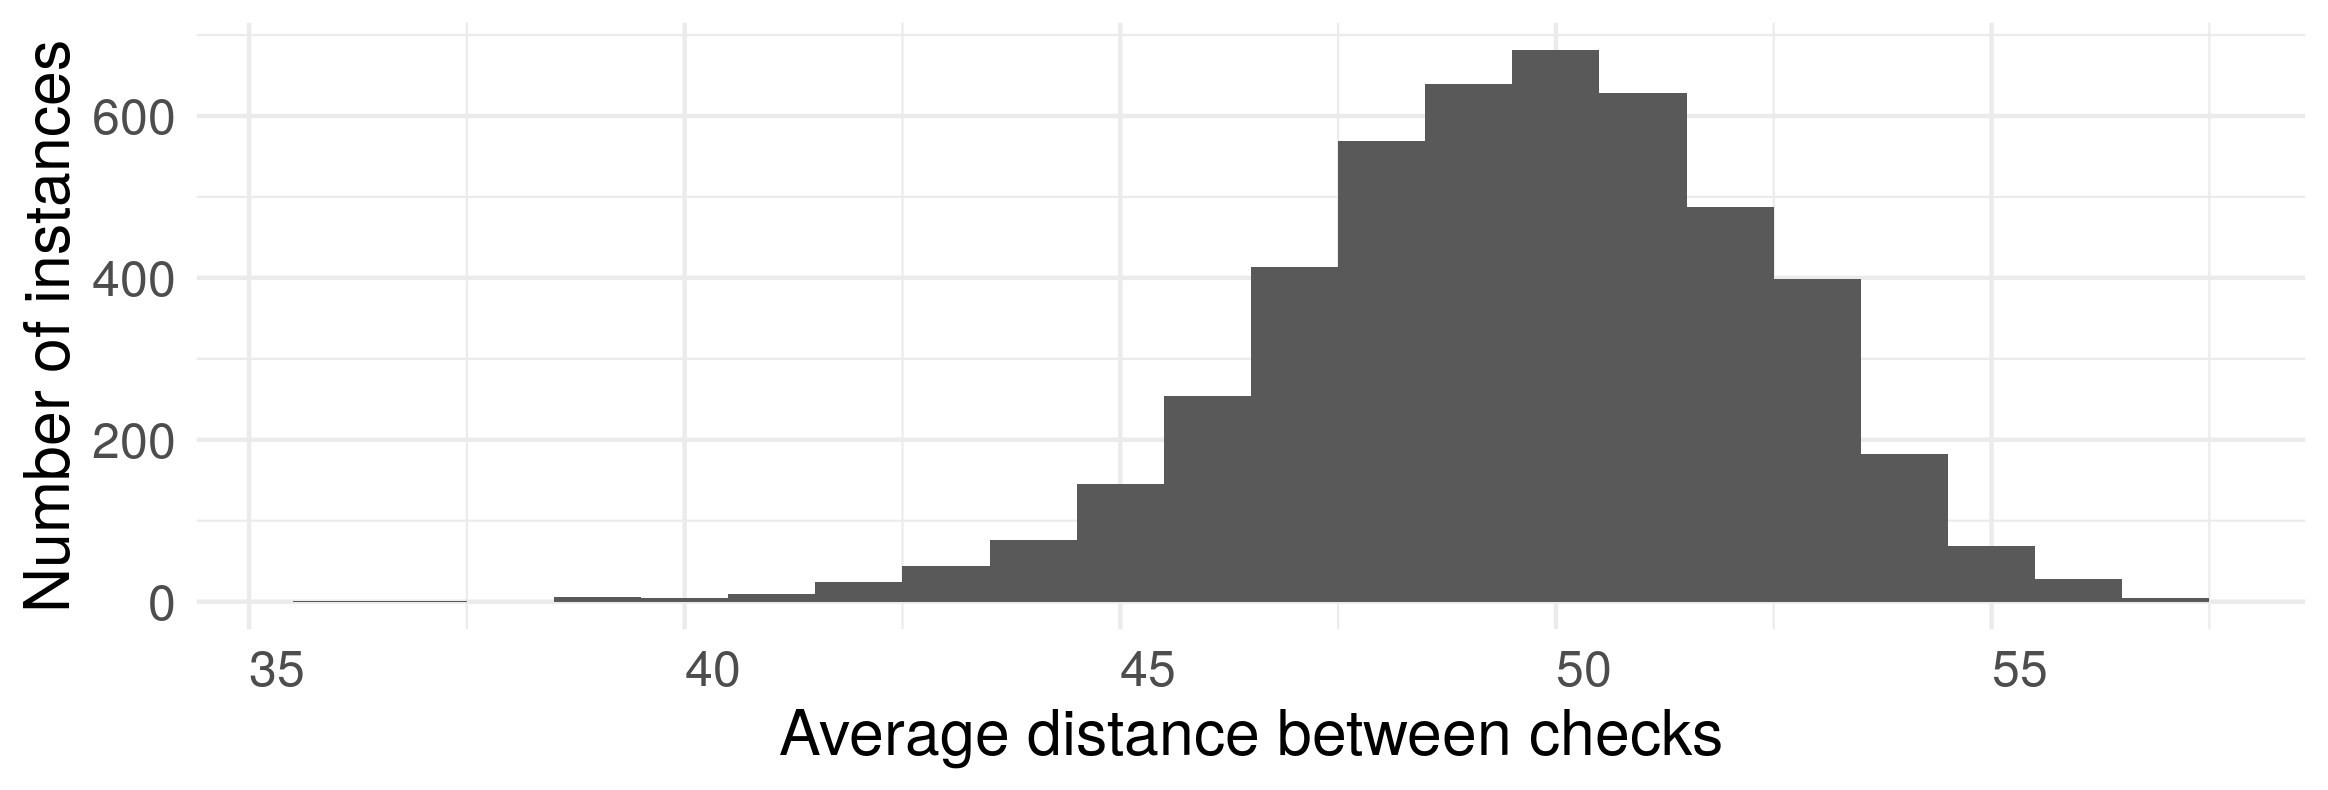
\includegraphics[height=0.3\linewidth]{images/distribution_mean_distances_IT000125_20190716}
  }

\end{frame}

\begin{frame}
\frametitle{\textbf{Input features}}

  \onslide<1->{  
    \begin{block}{\textbf{Mission related}}
      Max, average, variance of flight hours per period. Median period.
    \end{block}
  }
  \onslide<2->{  
    \begin{block}{\textbf{Fleet related}}
      Sum of initial status (rft).
    \end{block}
  }
  \onslide<3->{  
    \begin{block}{\textbf{Compatibility related}}
      Sum of all special mission flight hours.
    \end{block}
  }
\end{frame}

\begin{frame}
\frametitle{\textbf{Forecasting technique}}

  \onslide<1->{  
    \begin{block}{\textbf{Quantile regressions}}
      Upper bound and lower bound at 10\% and 90\%.
      \begin{equation*}
        \mu_{t'-t} \to [\hat{\mu}_{t'-t}^{lb}, \hat{\mu}_{t'-t}^{ub}]
     \end{equation*}
    \end{block}
  }
  \onslide<2->{  
  \begin{block}{\textbf{Training / test set}}
    of 5000 small instances solved to optimal and splitted: 70/30.
  \end{block}
  }

  % TODO: add prediction results
  % TODO: add prediction example
\end{frame}

\begin{frame}
\frametitle{\textbf{Applying learned-cuts}}

  \begin{block}{\textbf{Pattern filtering:}}
    \begin{equation*}
      D_{ip} \in [\hat{\mu}_{t'-t}^{lb} - tol, \hat{\mu}_{t'-t}^{ub} + tol] \rightarrow p \in \mathcal{P}_i 
    \end{equation*}
  \end{block}
  % TODO: add example
  \pause

  \begin{block}{\textbf{Pattern recycling:} with probabiliy $\alpha$}
    \begin{equation*}
      D_{ip} \notin [\hat{\mu}_{t'-t}^{lb} - tol, \hat{\mu}_{t'-t}^{ub} + tol] \land P(\alpha)  \rightarrow p \in \mathcal{P}_i 
    \end{equation*}
  \end{block}
\end{frame}

\begin{frame}
\frametitle{\textbf{Experiments}}
  \begin{itemize}

  \item Number of instances: medium (1000), large (1000) and very large
    (1000).
  \item Time limit at 3600 seconds.
  \item We seeded instance generation for better comparison.
  \item CPLEX running 1 thread.
  \end{itemize}

  Largest instances have 60 aircraft, 90 periods.
\end{frame}

\begin{frame}
\frametitle{\textbf{Results: performance}}

  % TODO: change colors
  % TODO: bigger picture
  \begin{itemize}[<+->]
    \item More solutions.
    \item Better solutions.
  \end{itemize}

  \only<1>{
    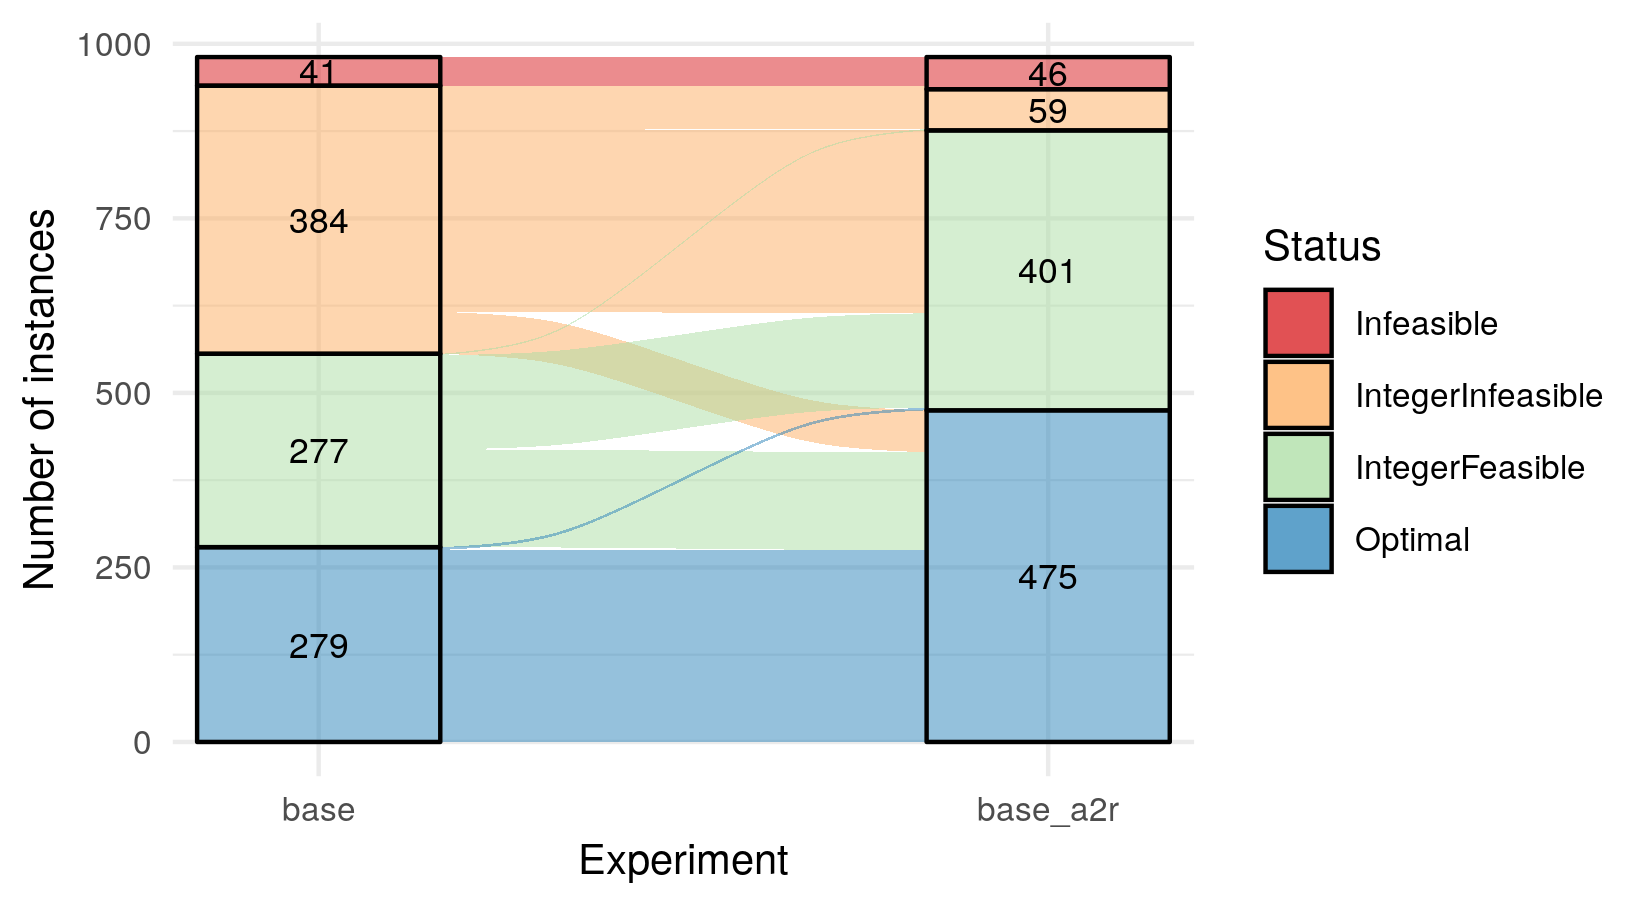
\includegraphics[width=0.8\linewidth]{images/transitions_base_2tasks.png}
  }
  \only<2>{
  % TODO: add one line at a time.
  % TODO: lines thicker and lines, not points
  % TODO: Time to solve instance (seconds)
    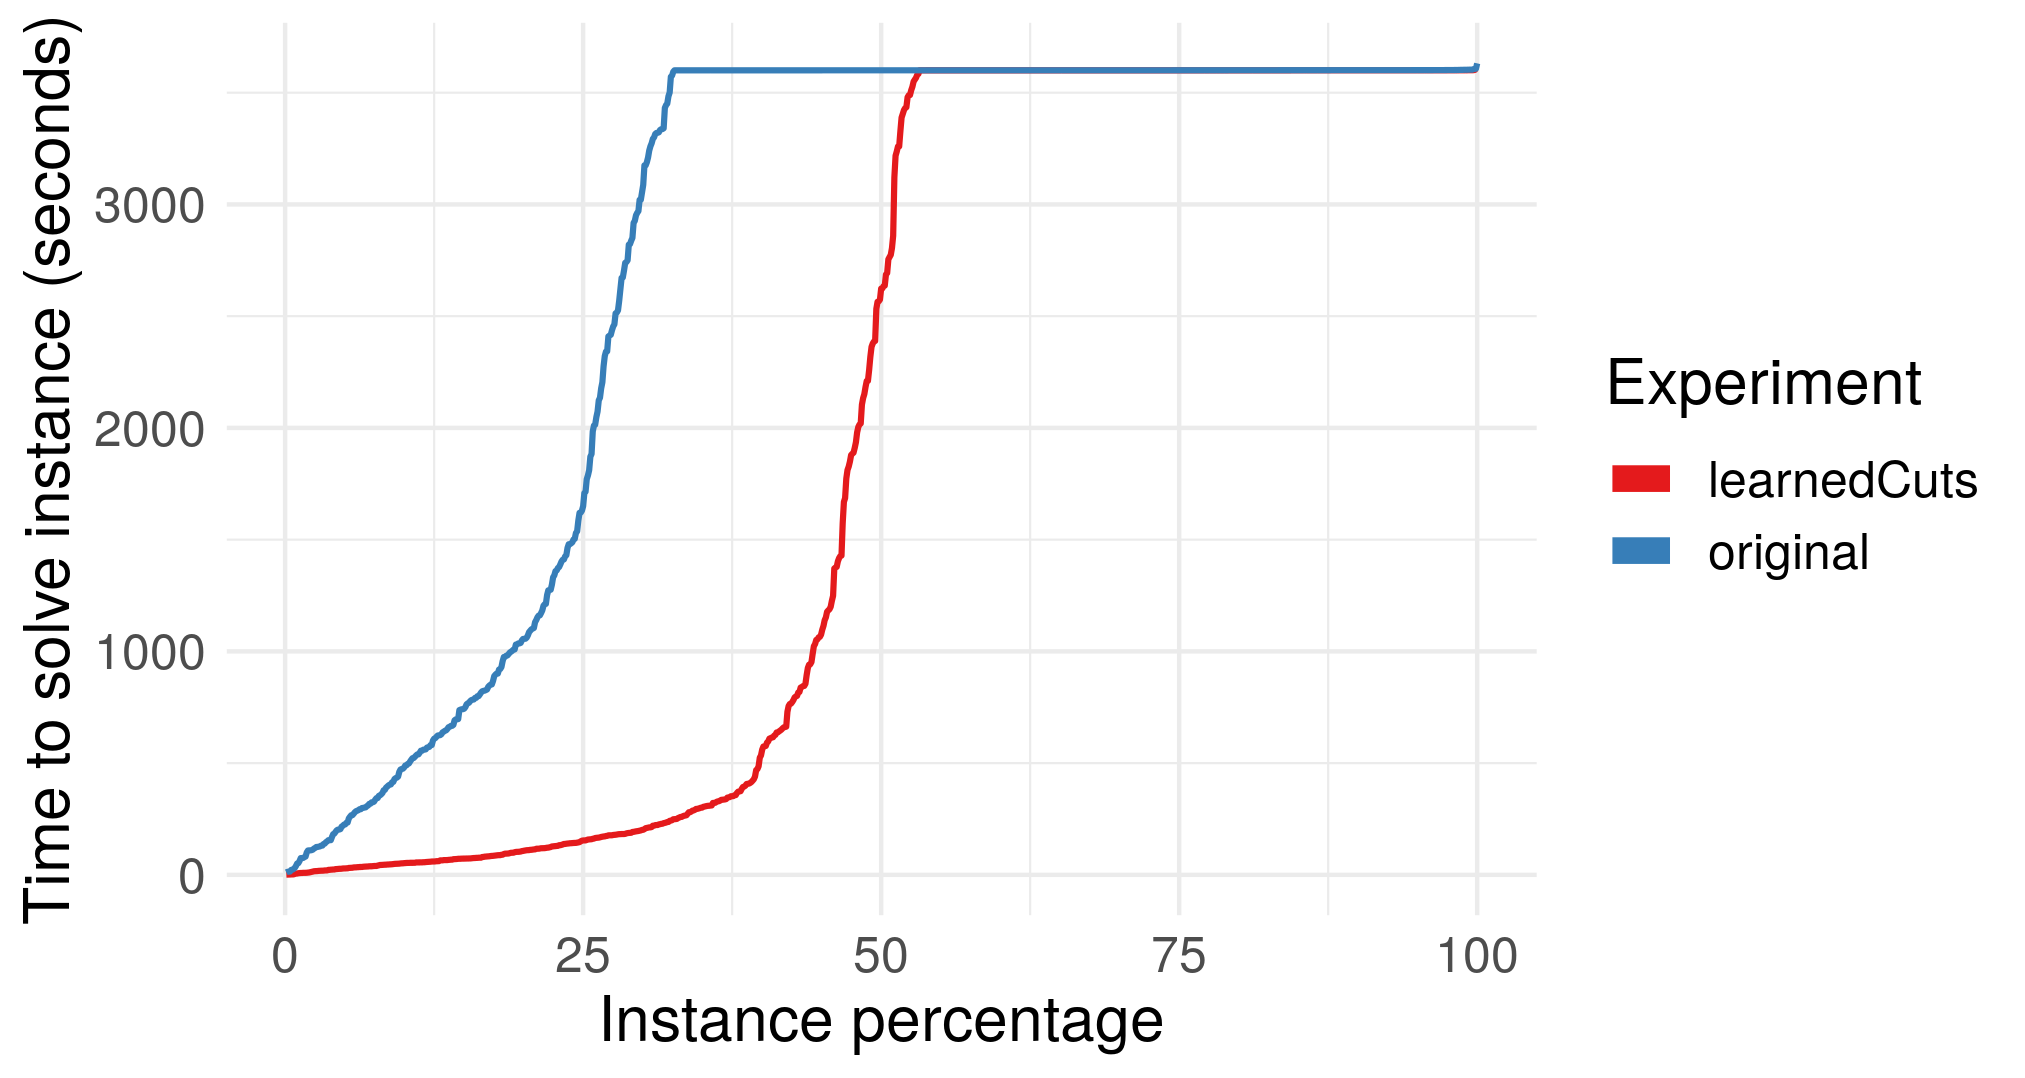
\includegraphics[width=0.8\linewidth]{images/time_performance_ordered_2tasks.png}
  }
\end{frame}

\begin{frame}
\frametitle{\textbf{Results: optimality}}

  \begin{itemize}[<+->]
    \item $\le$ 4\% loss of optimality.
    \item better predictions can improve this.
  \end{itemize}

  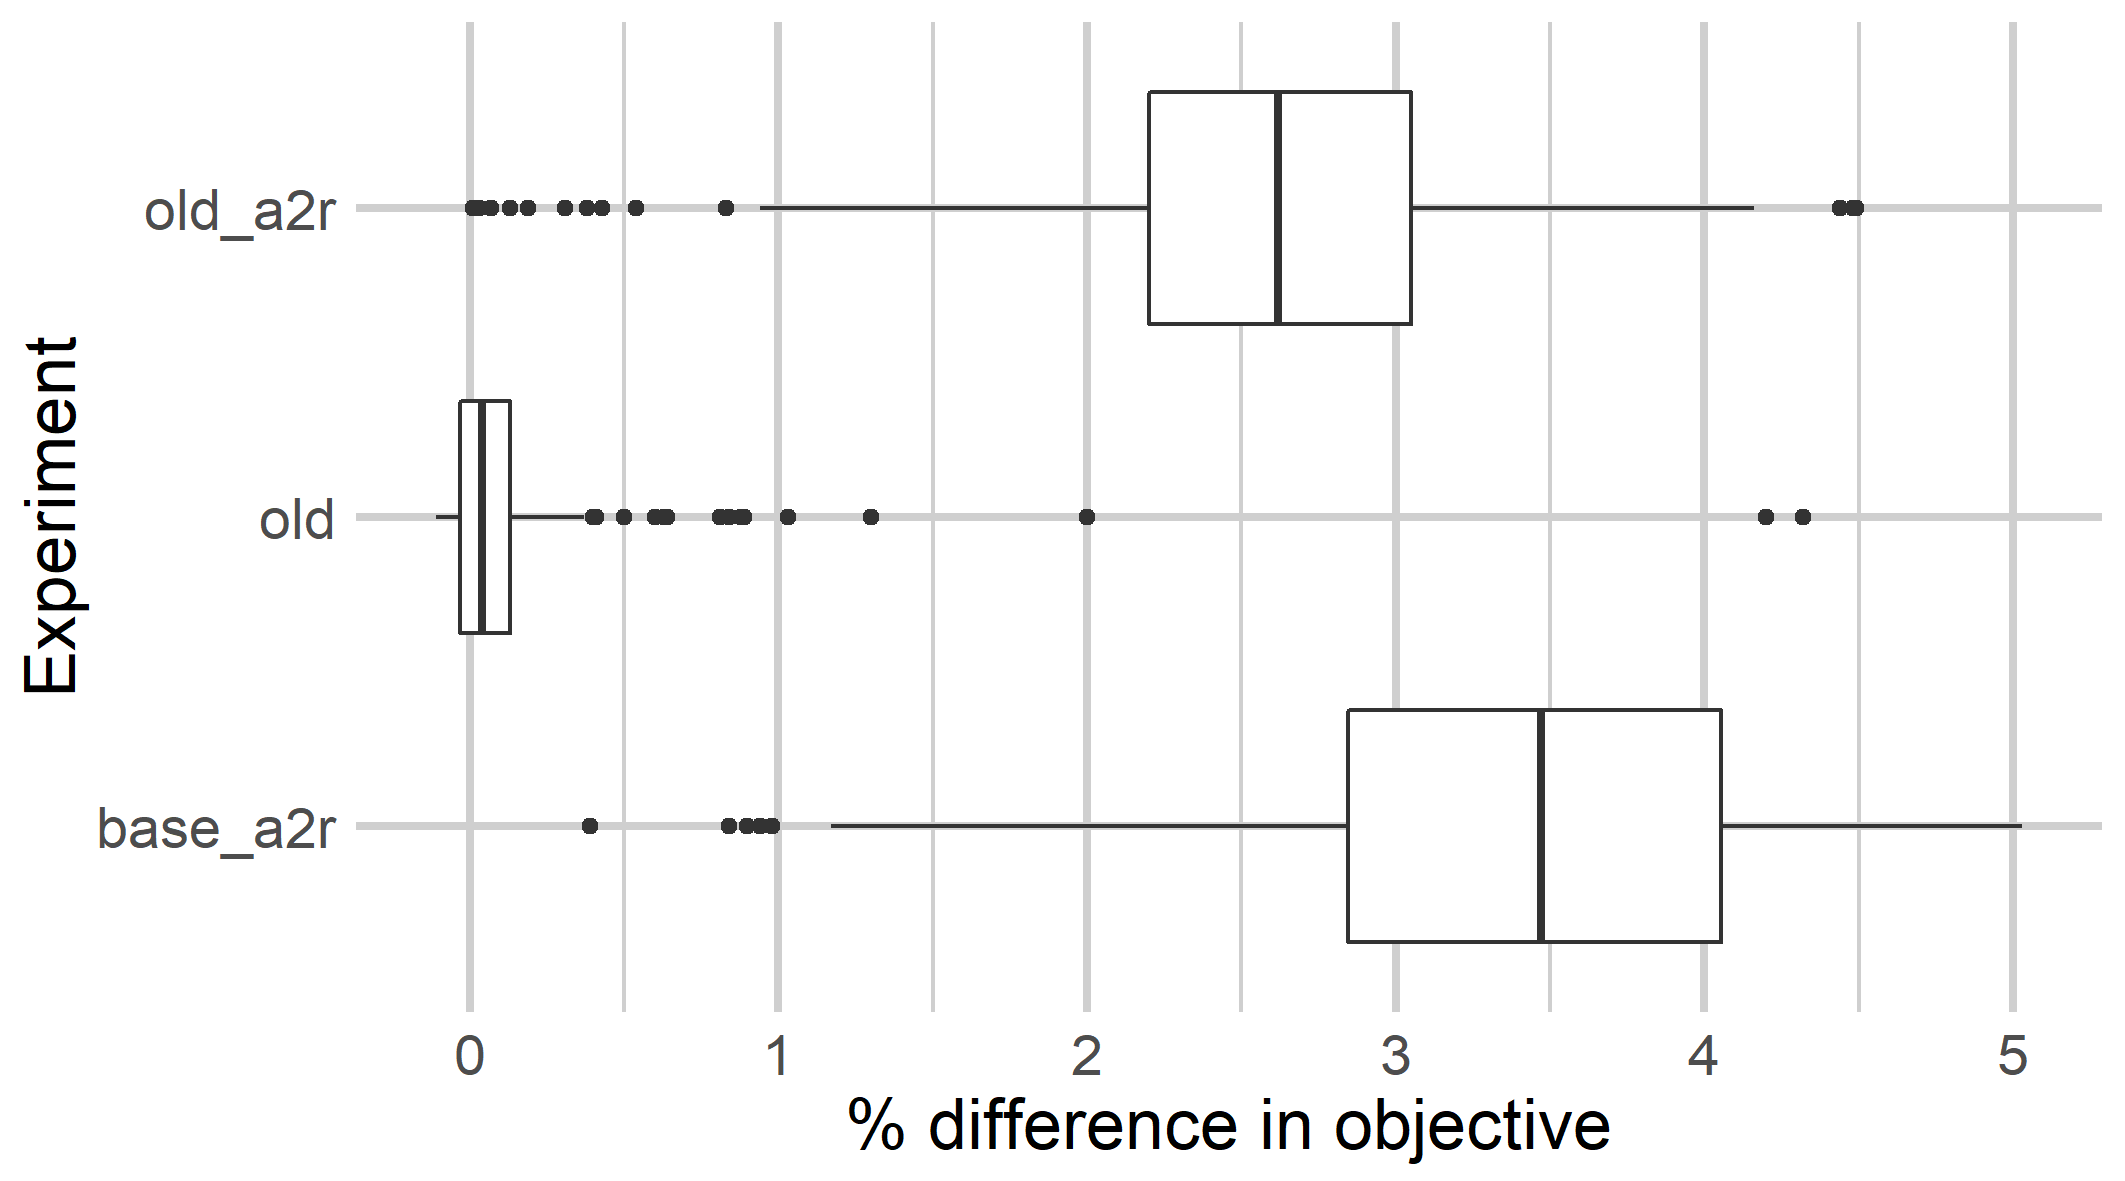
\includegraphics[width=0.8\linewidth]{images/quality_degradation_2tasks}

\end{frame}

\begin{frame}
\frametitle{\textbf{Preliminary conclusions}}
  \pause
  % TODO: check phrases
  \begin{block}{\textbf{Conclusions}}
    \begin{itemize}[<+->]
    \item \textbf{Supervised learning for optimization}
      provides good heuristic solutions.
    \item \textbf{MFMP application}
      shows the benefits of such an approach.
    \end{itemize}
  \end{block}  
  \pause
  \begin{block}{\textbf{Perspectives}}
    \begin{itemize}[<+->]
      \item \textbf{Generalize methodology} 
        to obtain a probability distribution for patterns, automatize feature extraction.
      \item \textbf{Combine it with other techniques} 
        to warm-start Column Generation, use a graph-based dynamic pattern generation.
    \end{itemize}
  \end{block}  
\end{frame}